\documentclass[aspectratio=169, 9pt]{beamer}
\usepackage[T2A]{fontenc}
\usepackage[utf8]{inputenc}
\usepackage[russian]{babel}
\usepackage{amsmath,amssymb,bm}
\usepackage{graphicx}
\usepackage{tikz}
\usepackage{booktabs}
\usepackage{array}
\usetikzlibrary{arrows.meta, positioning, shapes, calc, fit, matrix, backgrounds}

\usetheme{Ilmenau}
\usecolortheme{default}
\setbeamercolor{background canvas}{bg=white}
\setbeamercolor{normal text}{fg=black}
\setbeamercolor{frametitle}{fg=blue!80!black, bg=blue!5}
\setbeamercolor{title}{fg=white}
\setbeamercolor{item}{fg=blue!70}
\setbeamerfont{title}{size=\large, series=\bfseries}
\setbeamerfont{subtitle}{size=\normalsize}
\setbeamercolor{block title}{fg=white, bg=blue!60}
\setbeamercolor{block body}{bg=blue!5}
\setbeamertemplate{navigation symbols}{}
\setbeamertemplate{footline}{
  \leavevmode
  \hbox{
    \begin{beamercolorbox}[wd=.5\paperwidth,ht=2ex,dp=1ex,left]{author in head/foot}
      \hspace*{1em}\insertshortauthor
    \end{beamercolorbox}
    \begin{beamercolorbox}[wd=.5\paperwidth,ht=2ex,dp=1ex,right]{date in head/foot}
      \insertframenumber{} / \inserttotalframenumber\hspace*{1em}
    \end{beamercolorbox}}
  \vskip0pt
}

\title{Основы обработки естественного языка}
\subtitle{Нормализация, токенизация, типовые задачи и RNN-модели}
\author{Курс «Deep Learning»}
\date{2026}

\begin{document}

% Slide 1: Title
\begin{frame}
  \titlepage
\end{frame}

% Slide 2: Plan
\begin{frame}{Содержание}
  \begin{enumerate}
    \item Что такое обработка естественного языка?
    \item Токенизация и нормализация текста
    \item Типовые задачи NLP
    \item Рекуррентные нейронные сети в NLP
    \item Архитектуры LSTM, GRU и Seq2Seq
  \end{enumerate}
\end{frame}

% Slide 3: What is NLP
\begin{frame}{Что такое обработка естественного языка?}
  \begin{columns}[T]
    \begin{column}{0.5\textwidth}
      \begin{block}{Определение}
        NLP — область на стыке ИИ, лингвистики и информатики, изучающая методы взаимодействия компьютера и человеческого языка.
      \end{block}
      
      \textbf{История:} зародилась в 1950-х (тест Тьюринга). Правила и статистика сменились DL: word2vec, seq2seq, Transformer.
      
      \vspace{0.3em}
      \textbf{Конвейер NLP:}
      Предобработка $\to$ Векторизация $\to$ Модель
    \end{column}
    \begin{column}{0.5\textwidth}
      \begin{block}{Области применения}
        \begin{itemize}
          \item Чат-боты и голосовые помощники
          \item Поиск и ранжирование
          \item Машинный перевод
          \item Анализ тональности
          \item Аннотация текстов и NER
          \item Генерация текстов
        \end{itemize}
      \end{block}
    \end{column}
  \end{columns}
\end{frame}

% Slide 4: Tokenization
\begin{frame}{Токенизация}
  \begin{columns}[T]
    \begin{column}{0.45\textwidth}
      \begin{block}{Что такое токенизация?}
        Процесс разбиения текста на минимальные осмысленные единицы — \textbf{токены}: слова, подслова или символы.
      \end{block}
      
      \vspace{0.3em}
      Обязательный первый шаг NLP-конвейера. От качества токенизации зависит результат всех последующих этапов.
      
      \vspace{0.3em}
      \textbf{Пример:}
      \begin{center}
        \begin{tikzpicture}[font=\tiny]
          \node[draw, fill=blue!10, thick] (text) at (0,0) {\textquotedblleft Мама мыла раму\textquotedblright};
          \draw[->, thick] (0,-0.3) -- (0,-0.6);
          \node[draw, fill=green!10, thick] (tokens) at (0,-1.0) {[Мама] [мыла] [раму]};
          \node[font=\tiny] at (0,-1.4) {3 word-level токена};
        \end{tikzpicture}
      \end{center}
    \end{column}
    \begin{column}{0.55\textwidth}
      \textbf{Основные подходы:}
      
      \begin{block}{Word-level}
        Простое разделение по пробелам. Большой словарь ($10^5$--$10^6$). Проблема OOV (out-of-vocabulary).
      \end{block}
      
      \begin{block}{Subword (BPE, WordPiece)}
        Баланс размера словаря и покрытия. Решает OOV. Стандарт: BPE в GPT, WordPiece в BERT.
      \end{block}
      
      \begin{block}{Character-level}
        Минимальный словарь (алфавит). Но длинные последовательности, сложнее улавливать смысл.
      \end{block}
    \end{column}
  \end{columns}
\end{frame}

% Slide 5: Normalization
\begin{frame}{Нормализация текста}
  \begin{columns}[T]
    \begin{column}{0.5\textwidth}
      \textbf{1. Нижний регистр}
      
      «Москва» и «москва» — один токен. Уменьшает словарь.
      
      \vspace{0.5em}
      \textbf{2. Удаление стоп-слов}
      
      Предлоги, союзы, местоимения несут мало смысла и удаляются (для некоторых задач).
      
      \vspace{0.5em}
      \textbf{3. Очистка от спецсимволов}
      
      Удаление пунктуации, URL, HTML-тегов, цифрового мусора.
    \end{column}
    \begin{column}{0.5\textwidth}
      \textbf{4. Стемминг}
      
      Механическое отсечение окончаний. Быстро, но грубо.
      
      \textit{«бегущий» $\to$ «бегущ», «красивее» $\to$ «красив»}
      
      Алгоритмы: Портера, Snowball.
      
      \vspace{0.5em}
      \textbf{5. Лемматизация}
      
      Лингвистически корректное приведение к начальной форме (лемме) через словарь и морфологию.
      
      \textit{«бежал» $\to$ «бежать», «красивее» $\to$ «красивый»}
      
      Инструменты: NLTK, spaCy, pymorphy2 (русский).
    \end{column}
  \end{columns}
\end{frame}

% Slide 6: NLP Tasks
\begin{frame}{Типовые задачи NLP}
  \begin{columns}[T]
    \begin{column}{0.33\textwidth}
      \begin{block}{01 Классификация}
        Определение категории текста: спам, тематика, жанр.
      \end{block}
      \vspace{0.2em}
      \begin{block}{02 Тональность}
        Эмоциональная окраска текста: позитив/негатив/нейтрально.
      \end{block}
      \vspace{0.2em}
      \begin{block}{03 Машинный перевод}
        Автоматический перевод между языками.
      \end{block}
    \end{column}
    \begin{column}{0.33\textwidth}
      \begin{block}{04 NER}
        Named Entity Recognition: извлечение имён, дат, организаций.
      \end{block}
      \vspace{0.2em}
      \begin{block}{05 Генерация}
        Создание текста: саммаризация, диалоговые системы.
      \end{block}
      \vspace{0.2em}
      \begin{block}{06 QA}
        Question Answering: поиск ответа в заданном контексте.
      \end{block}
    \end{column}
    \begin{column}{0.33\textwidth}
      \begin{block}{07 Language Modeling}
        Предсказание следующего слова. Основа GPT.
      \end{block}
      \vspace{0.2em}
      \begin{block}{08 Парсинг}
        Синтаксический анализ, dependency parsing.
      \end{block}
      \vspace{0.2em}
      \begin{block}{09 Textual Entailment}
        Определение логической связи между текстами.
      \end{block}
    \end{column}
  \end{columns}
\end{frame}

% Slide 7: RNN in NLP
\begin{frame}{Рекуррентные нейронные сети в NLP}
  \begin{columns}[T]
    \begin{column}{0.45\textwidth}
      \begin{block}{Принцип работы RNN}
        Обрабатывают элементы последовательности по одному, сохраняя скрытое состояние (память), которое передаётся на каждом шаге.
      \end{block}
      
      \textbf{Почему RNN для языка?}
      Язык — последовательная структура. RNN учитывают порядок слов и могут моделировать контекст.
      
      \vspace{0.3em}
      \textbf{Ключевая формула:}
      \[
      h_t = f(W h_{t-1} + U x_t + b)
      \]
    \end{column}
    \begin{column}{0.55\textwidth}
      \begin{block}{Проблемы RNN}
        \textbf{Затухание и взрыв градиентов:} при длинных последовательностях базовая RNN теряет информацию о ранних элементах.
      \end{block}
      
      \textbf{LSTM (Hochreiter \& Schmidhuber, 1997):}
      \begin{itemize}
        \item Cell state как «конвейер» информации
        \item Forget gate: что забыть
        \item Input gate: что добавить
        \item Output gate: что вывести
      \end{itemize}
      
      \textbf{GRU:} упрощённая LSTM с двумя gate (reset, update). Быстрее, меньше памяти, сопоставимое качество.
    \end{column}
  \end{columns}
\end{frame}

% Slide 8: LSTM vs GRU
\begin{frame}{LSTM vs GRU}
  \begin{columns}[T]
    \begin{column}{0.5\textwidth}
      \begin{block}{LSTM}
        \begin{itemize}
          \item Три gate: forget, input, output
          \item Отдельная ячейка состояния (cell state)
          \item Больше параметров
          \item Лучше на длинных последовательностях
          \item Доминировал до появления Transformer
        \end{itemize}
      \end{block}
      
      \[
      \begin{aligned}
      f_t &= \sigma(W_f [h_{t-1}, x_t] + b_f) \\
      i_t &= \sigma(W_i [h_{t-1}, x_t] + b_i) \\
      \tilde{C}_t &= \tanh(W_C [h_{t-1}, x_t] + b_C) \\
      C_t &= f_t \odot C_{t-1} + i_t \odot \tilde{C}_t \\
      o_t &= \sigma(W_o [h_{t-1}, x_t] + b_o) \\
      h_t &= o_t \odot \tanh(C_t)
      \end{aligned}
      \]
    \end{column}
    \begin{column}{0.5\textwidth}
      \begin{block}{GRU}
        \begin{itemize}
          \item Два gate: reset, update
          \item Единое скрытое состояние (нет cell state)
          \item Меньше параметров
          \item Сопоставимое качество на коротких текстах
          \item Предпочтителен при ограниченных ресурсах
        \end{itemize}
      \end{block}
      
      \[
      \begin{aligned}
      r_t &= \sigma(W_r [h_{t-1}, x_t] + b_r) \\
      z_t &= \sigma(W_z [h_{t-1}, x_t] + b_z) \\
      \tilde{h}_t &= \tanh(W [r_t \odot h_{t-1}, x_t] + b) \\
      h_t &= (1-z_t) \odot h_{t-1} + z_t \odot \tilde{h}_t
      \end{aligned}
      \]
    \end{column}
  \end{columns}
\end{frame}

% Slide 9: Seq2Seq + Attention
\begin{frame}{Seq2Seq и механизм внимания}
  \begin{columns}[T]
    \begin{column}{0.45\textwidth}
      \begin{block}{Encoder-Decoder}
        Энкодер сжимает входную последовательность в вектор контекста, декодер генерирует выход. Используется в переводе и саммаризации.
      \end{block}
      
      \textbf{Проблема:} при длинных предложениях информация теряется при «упаковке» в один вектор.
      
      \vspace{0.3em}
      \textbf{Решение — Attention:}
      $$c_t = \textstyle\sum_{j=1}^{T} \alpha_{tj} h_j$$
      $$\alpha_{tj} = \frac{\exp(e_{tj})}{\sum_{k} \exp(e_{tk})}$$
      $$e_{tj} = a(s_{t-1}, h_j)$$
    \end{column}
    \begin{column}{0.55\textwidth}
      \centering
      \textbf{Seq2Seq + Attention}
      \begin{tikzpicture}[scale=0.4, font=\tiny]
        \node[draw, fill=blue!20] (e1) at (0,0) {Я};
        \node[draw, fill=blue!20] (e2) at (2.5,0) {изучаю};
        \node[draw, fill=blue!20] (e3) at (5,0) {НЛП};
        
        \node[draw, fill=red!20] (d1) at (2.5,-2) {I};
        \node[draw, fill=red!20] (d2) at (2.5,-4) {study};
        \node[draw, fill=red!20] (d3) at (2.5,-6) {NLP};
        
        % Attention weights
        \draw[->, blue!40, thick] (e1.south) -- (d1.north);
        \draw[->, blue!60, thick] (e2.south) -- (d2.north);
        \draw[->, blue!80, thick] (e3.south) -- (d3.north);
        \draw[->, blue!20, thick] (e2.south) to[out=-20,in=40] (d1.north);
        \draw[->, blue!20, thick] (e1.south) to[out=-60,in=20] (d2.north);
        
        \node[font=\tiny] at (0.5, -7) {Толщина линии = вес внимания};
      \end{tikzpicture}
      
      \vspace{0.3em}
      \textbf{Фундамент для Transformer:} внимание стало основой Transformer (Vaswani et al., 2017) — архитектуры GPT, BERT и всех современных LLM.
    \end{column}
  \end{columns}
\end{frame}

% Slide 10: RNN for Classification
\begin{frame}{RNN в задаче классификации текста}
  \begin{columns}[T]
    \begin{column}{0.5\textwidth}
      \begin{block}{Анализ тональности}
        RNN читает текст слово за словом, накапливая контекст. Последнее скрытое состояние содержит суть всего текста и подаётся на классификатор.
      \end{block}
      
      \textbf{BiLSTM-подход:}
      Двунаправленный LSTM обрабатывает текст слева направо и справа налево, захватывая полный контекст.
      
      \vspace{0.3em}
      \textbf{Pooling состояний:}
      Max-pooling по всем шагам — альтернатива последнему состоянию.
    \end{column}
    \begin{column}{0.5\textwidth}
      \centering
      \begin{tikzpicture}[scale=0.45, font=\tiny]
        % Words
        \node[draw, fill=blue!10] (w1) at (0,4) {Этот};
        \node[draw, fill=blue!10] (w2) at (2.5,4) {фильм};
        \node[draw, fill=blue!10] (w3) at (5,4) {велико-};
        \node[draw, fill=blue!10] (w4) at (7.5,4) {лепен};
        
        % Embeddings
        \node[draw, fill=green!20] (e1) at (0,2.7) {Emb};
        \node[draw, fill=green!20] (e2) at (2.5,2.7) {Emb};
        \node[draw, fill=green!20] (e3) at (5,2.7) {Emb};
        \node[draw, fill=green!20] (e4) at (7.5,2.7) {Emb};
        
        % LSTM chain
        \node[draw, fill=red!20] (l1) at (0,1.4) {LSTM};
        \draw[->] (0.8,1.4) -- (1.7,1.4);
        \node[draw, fill=red!20] (l2) at (2.5,1.4) {LSTM};
        \draw[->] (3.3,1.4) -- (4.2,1.4);
        \node[draw, fill=red!20] (l3) at (5,1.4) {LSTM};
        \draw[->] (5.8,1.4) -- (6.7,1.4);
        \node[draw, fill=red!20] (l4) at (7.5,1.4) {LSTM};
        
        % Connections
        \draw[->] (w1) -- (e1);
        \draw[->] (w2) -- (e2);
        \draw[->] (w3) -- (e3);
        \draw[->] (w4) -- (e4);
        \draw[->] (e1) -- (l1);
        \draw[->] (e2) -- (l2);
        \draw[->] (e3) -- (l3);
        \draw[->] (e4) -- (l4);
        
        % Classifier
        \draw[->] (l4.east) -- (8.5,1.4) -- (8.5,0) -- (3.75,0) -- (3.75,-0.7);
        \node[draw, fill=orange!20] (cls) at (3.75,-1.4) {Dense + Softmax};
        \node[font=\tiny, right] at (5.5,-1.4) {Позитив (0.92)};
      \end{tikzpicture}
      
      \vspace{0.3em}
      Пример: отзыв «Этот фильм великолепен!» $\to$ 4 шага LSTM $\to$ P(позитив) = 0.92
    \end{column}
  \end{columns}
\end{frame}

% Slide 11: NER
\begin{frame}{RNN в NER (BiLSTM-CRF)}
  \begin{columns}[T]
    \begin{column}{0.45\textwidth}
      \begin{block}{Архитектура BiLSTM-CRF}
        BiLSTM извлекает контекстные признаки для каждого токена. CRF-слой обеспечивает согласованность меток (B-PER не может идти после I-ORG).
      \end{block}
      
      \textbf{Почему двунаправленный?}
      Для NER нужен контекст с обеих сторон: «Маша работает в Яндекс».
      
      \vspace{0.3em}
      \textbf{BIO-тегирование:}
      \begin{itemize}
        \item \textbf{B} — начало сущности
        \item \textbf{I} — продолжение сущности
        \item \textbf{O} — не сущность
        \item PER — персона, ORG — организация, LOC — локация
      \end{itemize}
    \end{column}
    \begin{column}{0.55\textwidth}
      \centering
      \textbf{Пример:} «Иван работает в Газпром с 2010 года»
      
      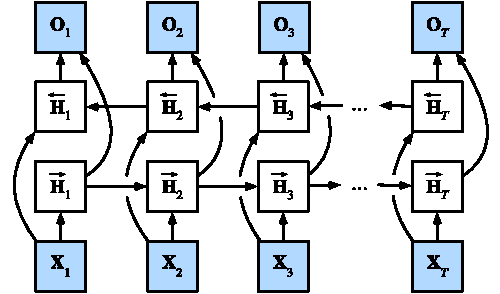
\includegraphics[width=0.85\textwidth]{images/birnn.pdf}
    \end{column}
  \end{columns}
\end{frame}

% Slide 12: Machine Translation

% Slide 12: Machine Translation
\begin{frame}{RNN в машинном переводе (Seq2Seq)}
  \begin{columns}[T]
    \begin{column}{0.5\textwidth}
      \begin{block}{Encoder-Decoder}
        Энкодер сжимает исходное предложение в последовательность скрытых состояний. Декодер генерирует перевод, используя механизм внимания.
      \end{block}
      
      \textbf{Внимание:} на каждом шаге декодер вычисляет веса для всех состояний энкодера. Взвешенная сумма фокусируется на релевантных частях.
      
      \textbf{Пример:} при переводе «Я изучаю нейронные сети» на шаге «study» внимание сфокусировано на «изучаю».
    \end{column}
    \begin{column}{0.5\textwidth}
      \centering
      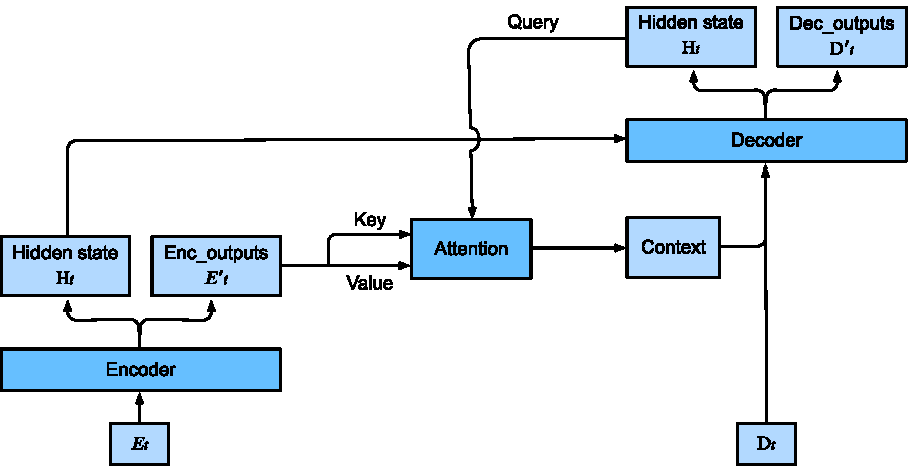
\includegraphics[width=0.95\textwidth]{images/seq2seq_att.pdf}
    \end{column}
  \end{columns}
\end{frame}

% Slide 13: Language Modeling
\begin{frame}{RNN в языковом моделировании и генерации}
  \begin{columns}[T]
    \begin{column}{0.48\textwidth}
      \begin{block}{Языковая модель}
        RNN предсказывает следующее слово. Обучается на корпусах, максимизируя вероятность правильного продолжения:
        $$P(w_1,\dots,w_T) = \prod P(w_t|w_{<t})$$
      \end{block}
      
      \textbf{Авторегрессия:} на генерации модель подаёт собственный выход как следующий вход.
      
      \textbf{Управление разнообразием:}
      \begin{itemize}
        \item Temperature $\tau$ — размывает распределение
        \item Top-K: семплинг из K лучших
        \item Top-P (nucleus): семплинг по кум. массе
      \end{itemize}
    \end{column}
    \begin{column}{0.55\textwidth}
      \centering
      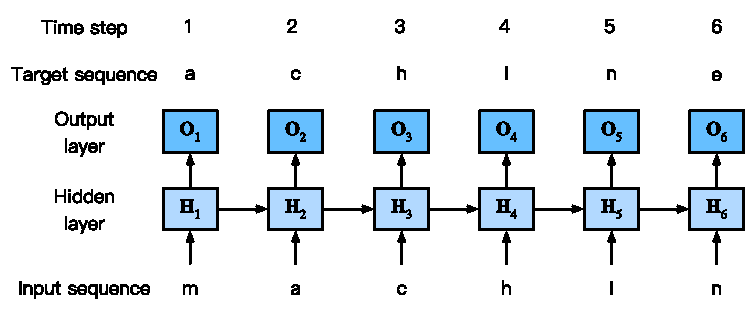
\includegraphics[width=0.85\textwidth]{images/rnn-train.pdf}
    \end{column}
  \end{columns}
\end{frame}

% Slide 14: Comparison
\begin{frame}{Сравнение подходов в NLP}
  \centering
  \begin{tabular}{lccc}
    \toprule
    \textbf{Критерий} & \textbf{Базовая RNN} & \textbf{LSTM / GRU} & \textbf{Transformer} \\
    \midrule
    Длинные зависимости & Слабо & Хорошо & \textbf{Отлично} \\
    Параллелизация & Нет & Нет & \textbf{Да} \\
    Скорость обучения & Быстрая & Средняя & Высокая (GPU) \\
    Качество & Низкое & Среднее & \textbf{SOTA} \\
    Потребление памяти & Мало & Средне & Много \\
    Типичное применение & Простые задачи & Перевод, NER & LLM, чат-боты \\
    \bottomrule
  \end{tabular}
  
  \vspace{1em}
  \begin{block}{Вывод}
    RNN/LSTM остаются актуальны для задач с ограниченными ресурсами, streaming-данных и real-time обработки. Transformer доминирует в качестве, но требует больше вычислительных ресурсов.
  \end{block}
\end{frame}

% Slide 15: Conclusion
\begin{frame}{Заключение}
  \begin{columns}[T]
    \begin{column}{0.5\textwidth}
      \textbf{Что мы узнали:}
      \begin{itemize}
        \item NLP-конвейер: токенизация $\to$ нормализация $\to$ модель
        \item Word, subword (BPE/WordPiece) и character-токенизация
        \item Стемминг vs лемматизация
        \item RNN, LSTM, GRU для последовательностей
        \item Seq2Seq + Attention для перевода
      \end{itemize}
    \end{column}
    \begin{column}{0.5\textwidth}
      \textbf{Применения RNN в NLP:}
      \begin{itemize}
        \item Классификация и тональность (BiLSTM)
        \item NER (BiLSTM-CRF)
        \item Машинный перевод (Seq2Seq + Attention)
        \item Языковое моделирование
        \item Генерация текста (авторегрессия)
      \end{itemize}
      
      \vspace{0.5em}
      \textbf{Дальше:} Transformer (лекция 06)
    \end{column}
  \end{columns}
\end{frame}

\end{document}
